% chktex-file 8
\documentclass[a4paper, 12pt]{report}
\usepackage[utf8]{inputenc}
\usepackage{graphicx}
\usepackage{setspace}
\usepackage{parskip}
\usepackage{mathptmx}
\newcommand{\Usefont}[1]{\fontfamily{#1}\selectfont}
\graphicspath{{figures/}}
\linespread{1.3}
\usepackage{titlesec}
\usepackage{url}
\usepackage{fancyvrb}
\usepackage{fvextra}
\usepackage{listings}
\usepackage{color} % for setting colors
\def\arraystretch{1.5}


% set the default code style for Python
\lstset{
    language=Python,
    stepnumber=1,
    showstringspaces=false,
    tabsize=1,
    breaklines=true,
    breakatwhitespace=false,
}

\usepackage[super,sort&compress]{natbib}
\titleformat{\chapter}[display]{\normalfont\fontsize{20pt}{24pt}\bfseries\centering}{CHAPTER \thechapter}{20pt}{\Large}
\titlespacing*{\chapter}{0pt}{-12pt}{24pt}

\titleformat{\section}
{\normalfont\bfseries\fontsize{12}{14}\selectfont\MakeUppercase}
{\thesection}
{1em}
{}

\titleformat{\subsection}
{\normalfont\bfseries\fontsize{12}{14}\selectfont}
{\thesubsection}
{1em}
{}

\usepackage{fancyhdr}
\pagestyle{fancy}
\fancyhf{}
\fancyhead[L]{ChatSNC\@: A Chatbot for College Website}
\fancyhead[R]{\thepage}
\fancyfoot[L]{Sree Narayana College, Kollam}
\setlength{\headheight}{15pt}

\renewcommand{\headrulewidth}{1 pt}
\renewcommand{\footrulewidth}{1 pt}

\renewcommand{\bibname}{References} 
\usepackage[nottoc]{tocbibind}

\setlength{\parindent}{3em}

\usepackage[]{lipsum}

\begin{document}
% These values are used thoroughout the report 
% please fill in the appropriate values in the brackets {}

\gdef\title{CHATSNC\@: A CHATBOT FOR COLLEGE WEBSITE } % Project title
%\gdef \author{Student Name}	 %student name
\gdef\dept{Physics and Computer Application} %Department
\gdef\degree{B.Sc Physics and Computer Application} %degree
\gdef\college{Sree Narayana College, Kollam} % Name of the College
\gdef\collegeplace{Kollam} % Location of the College
\gdef\studentA{Abil Asok} %Project batch member 1
\gdef\studentAroll{32821132002} % Project batch member 1 ktu id
\gdef\studentB{Indrajith R} %Project batch member 2
\gdef\studentBroll{32821132009} % Project batch member 2 ktu id

\gdef\studentC{Akshai Krishna S} %Project batch member 3
\gdef\studentCroll{32821132025} % Project batch member 3 ktu id

\gdef\studentD{Abhinav Manoj} %Project batch member 4
\gdef\studentDroll{32821132056} % Project batch member 4 ktu id

\gdef\guide{Prof.\ Project guide} %Project guide
\gdef\guidedes{Assistant Professor}%project guide designation

\gdef\guideco{Prof.\ Project coguide} %Project coguide
\gdef\guidecodes{Assistant Professor}%project coguide designation

\gdef\guideext{Prof.\ Project ext guide} %Project external organisation guide
\gdef\guideextdes{Engineer/Scientist}%project external guide designation
\gdef\guideextorg{External guide organization} % Project external guide organization

\gdef\projcordinatorA{Smt. Athira Rajendran}% Project coordinator 1 
\gdef\projcordinatorAdes{Assistant Professor}% Project coordinator 1 designation

\gdef\projcordinatorB{Smt.\ Surya S} % Project coordinator 2 
\gdef\projcordinatorBdes{Assistant Professor}% Seminar coordinator 2 designation

\gdef\hod{Smt. Asitha L. R} %Head of Department
\gdef\hoddes{Professor and Head} %HOD designation

\gdef\acadyear{2020 - 21} % Academic year
\gdef\month{June 2021} %Month of Report submission
\gdef\date{15-06-2021} %Date of signing the declaration

\bibliographystyle{IEEEtran}
% chktex-file 8
\newenvironment{coverpage}
\thispagestyle{empty}

\begin{titlepage}
	\begin{center}
		{\bfseries\large PROJECT REPORT}\\ \vspace*{25pt}
    {\bfseries\large\MakeUppercase{\dept}}\\ \vspace*{25pt}
    {\bfseries\large\MakeUppercase{\college}}\\ \vspace*{25pt}
    \begin{figure}[h!]
			\centerline{
\includegraphics[scale=0.6]{snc-logo}}
		\end{figure} \vspace*{25pt}
    {\bfseries\large\MakeUppercase{\title}}\\  \vspace*{25pt}
    {Submitted by\\} \vspace*{10pt}
     {\MakeUppercase{\studentA}} (\studentAroll)\\ \vspace*{7pt}
		 {\MakeUppercase{\studentB}} (\studentBroll)\\  \vspace*{7pt}
		 {\MakeUppercase{\studentC}} (\studentCroll)\\ \vspace*{7pt}
     {\MakeUppercase{\studentD}} (\studentDroll)\\ \vspace*{20pt}
     {Submitted in partial fulfilment of the Requirements for the award of\\\vspace*{5pt}B.Sc. Physics and Computer Applications degree,\\\vspace*{5pt}University of Kerala} \\\vspace*{5pt} 2021-2024
	\end{center}		
\end{titlepage}	


%==================================certificate1.tex================================
% To print name of only the seminar coordinator 1 in the certificate page


\newenvironment{certificate1}

	\newpage
  \thispagestyle{empty}
	\begin{center}	
		%\vspace{1.5cm}
		
		\textbf{SREE NARAYANA COLLEGE,\\ KOLLAM}	\\
		\textbf{University of Kerala}	
	\end{center}
	
	\begin{center}
		
\includegraphics[scale=0.4]{snc-logo}	
	\end{center}
	\begin{center}
		\textbf{CERTIFICATE}
	\end{center}
	
	This is to certify that the report titled \textbf{\title} is a bonafide record of the project done by \textbf{\studentA} (\studentAroll), \textbf{\studentB} (\studentBroll), \textbf{\studentC} (\studentCroll), and \textbf{\studentD} (\studentDroll) of the sixth semester \textbf{\degree} students under the guidance and supervision of \textbf{\projcordinatorA} and \textbf{\projcordinatorB} in partial fulfillment of the requirements for the award of the degree, \degree, at \college, affiliated with Kerala University.
	
	
	\begin{singlespace}
		\vspace*{1cm}
		\begin{table}[h!]
			\centering
			\begin{tabular}{p{3.5cm} p{5cm} p{5cm}} 
				\textbf{Dr.\ S.V. Manoj} & \textbf{\hod} & \textbf{\projcordinatorA} \\
				Principal & Head of the Department & Assistant Professor\\
				 & Physics and Computer\newline Application & Physics and Computer\newline Application
			\end{tabular}
		\end{table}
	\end{singlespace}
	\vspace{.5cm}
\noindent
\textbf{Submitted For University Exam Held On \ldots\ldots\ldots\ldots\ldots\ldots}

\vspace{.5cm}
	\begin{center}
		\begin{table}[h!]
			\centering
			\begin{tabular}{p{9cm} p{5cm}} 
				\textbf{External Examiner} & \textbf{Internal Examiner}
			\end{tabular}
		\end{table}
	\end{center}


\thispagestyle{empty}





%==================================declaration.tex================================
%
\newpage
\newenvironment{declaration}
\thispagestyle{empty}
\begin{center}
\vspace*{20pt}
\textbf{DECLARATION}\\
\vspace*{20pt}
\end{center}
We hereby declare that the project report {\bf{\title}}, submitted for partial fulfillment of the requirements for the award of degree of B.Sc. Physics and Computer Applications, University of Kerala
is a bonafide work done by us.\par
This submission represents our ideas in our own words and where ideas or words of others have been included, we have adequately and accurately cited and referenced the original sources.\par 
We also declare that we have adhered to ethics of academic honesty and integrity and have not misrepresented or fabricated any data or idea or fact or source in my submission. We understand that any violation of the above will be a cause for disciplinary action by the institute and/or the
University and can also evoke penal action from the sources which have thus not been properly cited or from whom proper permission has not been obtained. This report has not been previously formed the basis for the award of any degree, diploma or similar title of any other University.

\noindent \begin{minipage}{0.45\linewidth}
\begin{flushleft}
\vspace{2.5cm}

Kollam\\
Date:\end{flushleft} 
\end{minipage}
\hfill
\begin{minipage}{0.45\linewidth}
\begin{flushright}                                      
\vspace{1.5cm}

\textbf{\studentA}\\
\textbf{\studentB}\\
\textbf{\studentC}\\
\textbf{\studentD}\\


\end{flushright} 
\end{minipage}
\thispagestyle{empty}


\pagenumbering{roman}

\chapter*{Abstract}%
%\addcontentsline{toc}{chapter}{\numberline{}Abstract}%
\addcontentsline{toc}{chapter}{Abstract}%

Chatbots are becoming increasingly popular as a way
to provide information and assistance to users in various
domains. However, most chatbots rely on pre-defined scripts or large language models (LLMs) that may not have access to the latest or most relevant information for a specific context. In this project, we propose ChatSNC, a chatbot that uses Retrieval Augmented Generation (RAG) to chat with the website content of a college. RAG is a technique that combines information retrieval with text generation, allowing AI models to retrieve relevant information from a knowledge source and incorporate it into generated text. ChatSNC uses RAG to query the college website and generate responses that are grounded on the official and up-to-date information of the college. We demonstrate the effectiveness of ChatSNC by comparing it with a baseline chatbot that only uses an LLM without retrieval. We show that ChatSNC can provide more accurate, informative, and engaging responses than the baseline chatbot, and can handle a variety of user queries related to the college.


\thispagestyle{plain}

\chapter*{Acknowledgement}%
\addcontentsline{toc}{chapter}{Acknowledgement}%

%\newenvironment{acknowledgement}


\par We take this opportunity to express my deepest sense of gratitude and sincere thanks to everyone who helped us to complete this work successfully. We express our sincere thanks to \hod, Head of Department, \dept, \college\hspace*{2pt} for providing  us with all the necessary facilities and support.\par

We would like to express my sincere gratitude to the \projcordinatorA, \hspace*{2pt} department of \hspace*{2pt} \dept, \hspace*{2pt} \college\hspace*{2pt} for the support and co-operation.


\vspace*{30pt}
\begin{flushright}
	\textbf{\studentA}\\
	\textbf{\studentB}\\
	\textbf{\studentC}\\
	\textbf{\studentD}\\
\end{flushright}
\thispagestyle{plain}


\thispagestyle{empty}
\newpage

\tableofcontents
\listoffigures
\listoftables

\cleardoublepage\setcounter{page}{1}
\pagenumbering{arabic}


\chapter{INTRODUCTION}

\section{About the project}  



% chktex-file 8
\chapter{SYSTEM STUDY AND ANALYSIS}
\section{Existing System}  
The existing system in the realm of chatbots primarily revolves around Large Language Models (LLMs). These models have revolutionized the field of natural language processing (NLP), enabling machines to understand and generate human-like text at an unprecedented scale.

\subsection{Large Language Models (LLMs)}
LLMs are a type of artificial intelligence model designed to generate and understand human-like text by analyzing vast amounts of data. These foundational models are based on deep learning techniques and typically involve neural networks with many layers and a large number of parameters, allowing them to capture complex patterns in the data they are trained on.

The primary goal of an LLM is to understand the structure, syntax, semantics, and context of natural language, so it can generate coherent and contextually appropriate responses or complete given text inputs with relevant information. These models are trained on diverse sources of text data, including books, articles, websites, and other textual content, which enables them to generate responses to a wide range of topics.

Two popular LLMs are BERT (Bidirectional Encoder Representations from Transformers) developed by Google, and GPT-3 and GPT-4 developed by OpenAI\@. BERT marked a departure from the prevalent natural language processing (NLP) approach that relied on recurrent neural networks (RNNs). In contrast, BERT is trained bidirectionally, allowing it to gain a more comprehensive understanding of language context and flow compared to its unidirectional predecessors.

GPT-3, or Generative Pre-trained Transformer 3, has garnered significant attention for its remarkable capabilities in natural language understanding and generation1. It became publicly used when developed into GPT-3.5 for the creation of the conversational AI tool ChatGPT\@. The largest language model is now OpenAI's GPT-4, released in March 20231.

\subsection{ChatGPT}
ChatGPT is a chatbot developed by OpenAI and launched on November 30, 202234. Based on a large language model, it enables users to refine and steer a conversation towards a desired length, format, style, level of detail, and language4. It works by predicting the next word in a given text, based on the patterns it has learned from a massive amount of data during its training process5.

However, the effectiveness of these LLMs is hindered by concerns surrounding bias, inaccuracy, and toxicity, which limit their broader adoption and raise ethical concerns1. Despite these challenges, the existing system of LLMs has made significant strides in the field of AI and continues to evolve.
\subsection{Drawbacks of Existing System}
The existing system of Large Language Models (LLMs) and chatbots like ChatGPT, while impressive, have several limitations:
\begin{enumerate}
  \item \textbf{Limited Understanding}: LLMs may have a limited understanding of the context and meaning of the language they process. They lack the ability to understand nuances, cultural references, and context-dependent meanings. This can lead to inaccurate or inappropriate responses to certain inputs. For example, they might not understand the difference between a genuine request for information and a rhetorical question, leading to responses that may seem out of place or irrelevant.
  \item \textbf{Incorrect Answers}: LLMs can make mistakes, including grammatical, mathematical, factual, and reasoning errors. They sometimes struggle to acknowledge their lack of knowledge and instead fabricate plausible-sounding answers. This can be problematic in situations where accurate information is crucial, such as in academic or professional settings. For instance, an LLM might generate an incorrect mathematical solution or provide outdated or incorrect factual information.
  \item \textbf{Biased Answers}: LLMs can reflect the biases present in their training data. This can lead to the perpetuation of stereotypes and biases. For example, if the training data contains gender biases, the LLM might generate responses that reinforce these biases. This is a significant issue as it can contribute to the spread of harmful stereotypes and discrimination.
  \item \textbf{Lack of Human Insight:}: LLMs lack the ability for genuine expression. They cannot produce content that touches people emotionally on the same level as a human can, as they have no actual thoughts or feelings. This means that while they can generate text that might seem insightful or empathetic, it's important to remember that these are simply outputs based on patterns in the data they were trained on, not genuine expressions of emotion or understanding.
  \item \textbf{Lack of Transparency}: LLMs like GPT-3 are highly complex and difficult to interpret. This makes it challenging to understand how they arrive at certain outputs. This lack of transparency can make it difficult to troubleshoot or improve the models, and it can also raise ethical concerns about accountability and fairness.
  \item \textbf{Ethical Concerns}: The use of LLMs raises ethical concerns, particularly around the generation of misinformation and the potential misuse of the technology. For example, they could be used to generate fake news or deceptive content, which could have serious societal implications.
  \item \textbf{Environmental Impact}: Training and running LLMs require significant computational resources, which can have a substantial environmental impact. The energy required to train these models and generate responses can contribute to carbon emissions, which is a significant concern given the ongoing climate crisis.

\end{enumerate}

\section{Proposed System}
\textbf{Retrieval-Augmented Generation (RAG)}\cite{lewis2021retrievalaugmented} is a method that combines the strengths of both retrieval-based and generative models for natural language understanding and generation.

\subsection{Working of RAG}
The working of RAG can be divided into several steps:
\begin{enumerate}
  \item \textbf{Data Loading}: The first step involves loading the dataset which is used for training the model. This dataset typically consists of a large number of documents or dialogues which provide the model with a diverse range of language patterns and structures. The data is usually preprocessed and tokenized before being fed into the model
  \item \textbf{Document Retrieval}: Once the data is loaded, the next step is document retrieval. When a new input (like a user query) is received, the model retrieves a set of relevant documents from the dataset. This is done using a dense retrieval method, which uses semantic similarity to find the most relevant documents. The semantic similarity is calculated using vector representations of the documents and the query. These vector representations are usually obtained using methods like Word2Vec or BERT, which convert the text into high-dimensional vectors. The similarity between the vectors is then calculated using methods like cosine similarity.
  \item \textbf{Question-Answering}: After the relevant documents are retrieved, a question-answering model is used. This model takes the user query and the retrieved documents as input, and generates a set of candidate responses. The question-answering model is usually a transformer-based model, which uses attention mechanisms to understand the context of the query and the documents, and generate relevant responses.
  \item \textbf{Response Generation}: Finally, a generative model is used to generate a response. This model takes the candidate responses from the previous step and generates a final response. This response is generated in a way that it is contextually relevant to the user query and is fluent and coherent in terms of language. The generative model is also usually a transformer-based model, which uses the context of the conversation and the candidate responses to generate a response.
\end{enumerate}
The key aspect of RAG is that it combines the strengths of retrieval-based and generative models. The retrieval component allows the model to leverage the information in the dataset, while the generative component allows the model to generate fluent and contextually relevant responses.
\subsection{Advantages of Proposed System}
Retrieval-Augmented Generation (RAG) offers several advantages that help overcome the limitations of traditional large language models (LLMs) like GPT-3. Here are some key advantages:
\begin{enumerate}
  \item \textbf{Contextual Understanding}: RAG models have a better understanding of the context as they retrieve relevant documents from a dataset before generating a response. This allows them to provide more accurate and contextually relevant responses compared to traditional LLMs, which generate responses based solely on the input they receive.
  \item \textbf{Information Retrieval}: One of the limitations of traditional LLMs is their inability to retrieve and leverage external information during the conversation. RAG models overcome this by retrieving relevant documents from a dataset, allowing them to provide responses that are not only based on the model's training data but also on the specific information present in the retrieved documents.
  \item \textbf{Dynamic Knowledge Update}: Traditional LLMs are trained on a static dataset, and their knowledge is fixed at the time of training. In contrast, RAG models can dynamically update their knowledge by retrieving information from a constantly updated dataset. This allows them to provide up-to-date information in their responses.
  \item \textbf{Scalability}: RAG models are scalable as they separate the retrieval and generation processes. This allows them to handle larger datasets and generate more diverse responses. In contrast, traditional LLMs may struggle with scalability as they need to process the entire dataset for every input.
  \item \textbf{Efficiency}: By separating the retrieval and generation processes, RAG models can efficiently handle complex tasks. They first narrow down the relevant information through retrieval and then focus on generating a response based on the retrieved information. This makes them more efficient compared to traditional LLMs, which need to consider the entire dataset while generating a response.
\end{enumerate}
In conclusion, RAG offers a robust solution for building chatbots by effectively combining the strengths of retrieval-based and generative models. It leverages the power of recent advancements in AI and LLMs to provide accurate, contextually relevant, and up-to-date responses.
\section{Preparation of Requirements}
The development of the chatbot for the college website required careful planning and preparation. The requirements were gathered and analyzed to ensure that the chatbot would meet the needs of the users and align with the goals of the project. The following are the key requirements that were identified:
\subsection{Functional Requirements}
\begin{enumerate}
  \item \textbf{User Input Processing}: The chatbot should be able to process user inputs in the form of text queries, understand the intent behind the queries, and generate appropriate responses.
  \item \textbf{Information Retrieval}: The chatbot should be able to retrieve relevant information from the college website to provide accurate and up-to-date responses to user queries.
  \item \textbf{Response Generation}: The chatbot should be able to generate fluent and contextually relevant responses based on the user queries and the retrieved information.
  \item \textbf{User Interaction}: The chatbot should be able to engage in natural and meaningful conversations with users, providing a seamless and user-friendly experience.
  \item \textbf{Multi-turn Conversations}: The chatbot should be able to handle multi-turn conversations, where the user can ask follow-up questions or continue the conversation on a specific topic.
  \item \textbf{Error Handling}: The chatbot should be able to handle errors and provide appropriate responses when it encounters queries that it cannot understand or process.
  \item \textbf{User and Chat History Management}: The chatbot should be able to handle user data and chat history, storing them securely in the database for future reference.
\end{enumerate}
\subsection{Non-Functional Requirements}
\begin{enumerate}
  \item \textbf{Accuracy}: The chatbot should provide accurate and reliable information to users, ensuring that the responses are based on the most up-to-date information available on the college website.
  \item \textbf{Performance}: The chatbot should be able to process user queries and generate responses in a timely manner, providing a responsive and efficient user experience.
  \item \textbf{Security}: The chatbot should adhere to data privacy and security standards, ensuring that user data is protected and handled in a secure manner.
  \item \textbf{User Experience}: The chatbot should provide a seamless and intuitive user experience, with a user-friendly interface and natural language interactions.
\end{enumerate}
\subsection{Technical Requirements}
\begin{enumerate}
  \item \textbf{Frontend}: The chatbot's user interface should be built using Vue.js to ensure a responsive and interactive user experience.
  \item \textbf{Backend}: The backend should be built using FastAPI to handle requests and responses efficiently. The backend should also incorporate the Llama index for handling the LLM and RAG\@.
  \item \textbf{Database}: PostgreSQL should be used as the database to store and manage data due to its robustness and reliability. The database should have tables for users and chat history.
\end{enumerate}
\section{Feasibility Study}
Before the commencement of the project, a feasibility study was conducted to assess the viability of the chatbot project for the college website. The study focused on the following areas:
\subsection{Technical Feasibility}
The project is technically feasible as it leverages Vue.js for frontend development, which is known for its simplicity and flexibility. FastAPI, a modern, fast (high-performance), web framework for building APIs is used for backend development. It has a significant advantage in terms of speed and ease of use. The Llama index is used for handling the LLM and RAG, and PostgreSQL, a powerful, open-source object-relational database system, is used for data storage. Additionally, OpenAI's GPT-3.5 and their embedding model are used for language understanding and generation, which are known for their high performance and accuracy. These technologies are well-documented and widely supported, which makes the development process efficient and manageable.
\subsection{Economic Feasibility}
From an economic perspective, the project is feasible as the technologies used (Vue.js, FastAPI, Llama index, PostgreSQL) are open-source and free to use. While OpenAI's models are not open-source, they come at a reasonable cost.
\subsection{Operational Feasibility}
The proposed chatbot is operationally feasible as it is designed to interact with users in a natural, conversational manner, and assist them in navigating the college website and finding the information they need. It can handle user data and chat history, storing them securely in the database for future reference.
\subsection{Legal and Ethical Feasibility}
The project complies with all relevant data protection and privacy laws. User data is handled securely, and privacy is maintained.
\subsection{Schedule Feasibility}
Given the scope of the project and the technologies used, the development of the chatbot is achievable within the proposed timeline.
\section{Data Flow Diagram}
To be filled 


\chapter{System Design}

\section{Algorithms}


% chktex-file 44
% chktex-file 18
% chktex-file 36
% chktex-file 37
% chktex-file 11
% chktex-file 38
% chktex-file 25
% chktex-file 28
% chktex-file 35
% chktex-file 12
% chktex-file 16
% chktex-file 32
% chktex-file 26
% chktex-file 8


\chapter{System Coding and Unit Testing}

\section{System Coding}

\subsection{Program List}


\begin{table}[h!]
  \centering
  \caption{Program List}
  \vspace*{10pt}
  \begin{tabular}{|p{4cm}|p{8cm}|}
    \hline
    \multicolumn{1}{|c|}{\textbf{Program Name}} & \multicolumn{1}{c|}{\textbf{Description}}\\ \hline
    snc\_chat.py & Chat engine for the ChatSNC application\\ \hline
    load\_index.py & Load documents as vector into the vector database\\ \hline
    main.py & Main FastAPI application\\ \hline
    auth.py & Authentication routes\\ \hline
    chatsnc.py & ChatSNC routes\\ \hline
    user.py & User routes\\ \hline
  \end{tabular}
\end{table}

\subsection{Program Code}
  
\textbf{snc\_chat.py}

\begin{Verbatim}[breaklines=true, breakanywhere=true]
import chromadb
from llama_index.indices import VectorStoreIndex
from llama_index.vector_stores import ChromaVectorStore
from llama_index.storage.storage_context import StorageContext
from llama_index import ServiceContext, set_global_service_context
from llama_index.llms import Cohere
from llama_index.embeddings import OpenAIEmbedding

from llama_index.llms import Ollama

from ...config import settings
import os

os.environ["OPENAI_API_KEY"] = settings.openai_api_key

db = chromadb.PersistentClient(path="./app/engine/chatsnc/chroma_db")

# get collection
chroma_collection = db.get_collection("college_laws")

# assign chroma as the vector_store to the context
vector_store = ChromaVectorStore(chroma_collection=chroma_collection)
storage_context = StorageContext.from_defaults(vector_store=vector_store)

# load your index from stored vectors
index = VectorStoreIndex.from_vector_store(
    vector_store,
    storage_context=storage_context,
)

def chat(query, chat_history):
    """
    Perform a chat using the given query and chat history.

    Args:
        query (str): The query to be used for the chat.
        chat_history (list): The chat history as a list.

    Returns:
        str: The response generated by the chat engine.
    """
    global index
    chat_engine = index.as_chat_engine(streaming=True)

    return chat_engine.stream_chat(query, chat_history=chat_history)  
\end{Verbatim}
\
\\
\textbf{load\_index.py}

\begin{Verbatim}[breaklines=true, breakanywhere=true]
"""
This script loads documents into a vector store index using the ChromaDB library.

The script performs the following steps:
1. Imports necessary libraries and modules.
2. Sets the OpenAI API key as an environment variable.
3. Initializes an OpenAIEmbedding model for text embedding.
4. Sets the service context for the vector store index.
5. Loads documents from a specified directory using the SimpleDirectoryReader.
6. Initializes a ChromaDB client and creates a collection.
7. Assigns ChromaVectorStore as the vector store to the storage context.
8. Creates a vector store index from the loaded documents using the storage context.
"""

import chromadb
from llama_index import VectorStoreIndex, SimpleDirectoryReader, download_loader
from llama_index.vector_stores import ChromaVectorStore
from llama_index.storage.storage_context import StorageContext
from llama_index import ServiceContext, set_global_service_context
from llama_index.embeddings import OpenAIEmbedding
import os
import getpass

os.environ["OPENAI_API_KEY"] = getpass.getpass("OpenAI API Key:")

embed_model = OpenAIEmbedding(model="text-embedding-3-small")

service_context = ServiceContext.from_defaults(embed_model=embed_model)

set_global_service_context(service_context)

# load some documents
UnstructuredReader = download_loader("UnstructuredReader")
dir_reader = SimpleDirectoryReader(
    "./data",
    file_extractor={
        ".pdf": UnstructuredReader(),
        ".html": UnstructuredReader(),
        ".eml": UnstructuredReader(),
    },
)
documents = dir_reader.load_data()

# initialize client, setting path to save data
db = chromadb.PersistentClient(path="./chroma_db")

# create collection
chroma_collection = db.get_or_create_collection("college_laws")

# assign chroma as the vector_store to the context
vector_store = ChromaVectorStore(chroma_collection=chroma_collection)
storage_context = StorageContext.from_defaults(vector_store=vector_store)

# create your index
index = VectorStoreIndex.from_documents(documents, storage_context=storage_context)
\end{Verbatim}

\
\\
\textbf{main.py}

\begin{Verbatim}[breaklines=true, breakanywhere=true]
from .config import settings

if settings.app == "prod":
    __import__("pysqlite3")
    import sys

    sys.modules["sqlite3"] = sys.modules.pop("pysqlite3")
from fastapi import FastAPI
from .routers import user, auth, chatsnc
from fastapi.middleware.cors import CORSMiddleware
from . import models
from .database import engine


# models.Base.metadata.create_all(bind=engine)

app = FastAPI()

origins = [
    "http://chatsnc.vercel.app",
    "https://chatsnc.vercel.app",
    "http://localhost:5173",
]

app.add_middleware(
    CORSMiddleware,
    allow_origins=origins,
    allow_credentials=True,
    allow_methods=["*"],
    allow_headers=["*"],
)

app.include_router(user.router)
app.include_router(auth.router)
app.include_router(chatsnc.router)
\end{Verbatim}

\
\\
\textbf{auth.py}

\begin{Verbatim}[breaklines=true, breakanywhere=true]
from ..database import get_db
from .. import models, schemas, utils, oauth2
from sqlalchemy.orm import Session
from fastapi import status, HTTPException, Depends, APIRouter
from fastapi.security.oauth2 import OAuth2PasswordRequestForm

router = APIRouter(
    tags=["Authentication"],
)


@router.post("/login", status_code=status.HTTP_200_OK, response_model=schemas.Token)
def login(
    user_credentials: OAuth2PasswordRequestForm = Depends(),
    db: Session = Depends(get_db),
):
    user = (
        db.query(models.User)
        .filter(models.User.email == user_credentials.username)
        .first()
    )
    if not user:
        raise HTTPException(
            status_code=status.HTTP_403_FORBIDDEN, detail="Invalid credentials"
        )
    if not utils.verify(user_credentials.password, user.password):  # type: ignore
        raise HTTPException(
            status_code=status.HTTP_403_FORBIDDEN, detail="Invalid credentials"
        )

    access_token = oauth2.create_access_token(data={"user_id": user.id})
    return {"access_token": access_token, "token_type": "bearer", "user": user}

\end{Verbatim}
\
\\
\textbf{chatsnc.py}

\begin{Verbatim}[breaklines=true, breakanywhere=true]
from .. import models, schemas
from ..database import get_db
from sqlalchemy import func
from sqlalchemy.orm import Session
from typing import List
from fastapi import status, HTTPException, Depends, Response, APIRouter
from .. import oauth2
from typing import List, Optional
from ..engine.chatsnc import snc_chat
from pydantic import BaseModel
import asyncio
from fastapi.responses import StreamingResponse
from llama_index.llms import ChatMessage, MessageRole
import json
from fastapi.encoders import jsonable_encoder

router = APIRouter(
    prefix="/chat",
    tags=["ChatSNC"],
)


async def astreamer(generator):
    try:
        for i in generator:
            yield (i)
            await asyncio.sleep(0.1)
    except asyncio.CancelledError as e:
        print("cancelled")


@router.post("/generate", status_code=status.HTTP_201_CREATED)
def generate_chat(
    query: str,
    history: List[schemas.History],
    db: Session = Depends(get_db),
    user: schemas.UserOut = Depends(oauth2.get_current_user),
):
    chat_history = [
        ChatMessage(
            role=MessageRole.USER,
            content="Hello assistant, we are having a insightful discussion about Rules of SN College today.",
        ),
        ChatMessage(role=MessageRole.ASSISTANT, content="Okay, sounds good."),
    ]
    for h in history:
        chat_history.append(ChatMessage(role=h.role, content=h.content))
    response = snc_chat.chat(query, chat_history)
    return StreamingResponse(astreamer(response.response_gen), media_type="text/plain")


@router.post(
    "/", status_code=status.HTTP_201_CREATED, response_model=schemas.ChatCreateOut
)
def create_chat(
    db: Session = Depends(get_db),
    user: schemas.UserOut = Depends(oauth2.get_current_user),
):
    new_chat = models.Chat(
        user_id=user.id,
    )
    db.add(new_chat)
    db.commit()
    db.refresh(new_chat)
    return new_chat


@router.put("/{id}", status_code=status.HTTP_200_OK)
def update_chat(
    id: int,
    history: List[schemas.HistoryOut],
    db: Session = Depends(get_db),
    user: schemas.UserOut = Depends(oauth2.get_current_user),
):
    chat_str = json.dumps(jsonable_encoder(history))

    chat_query = db.query(models.Chat).filter(models.Chat.id == id)
    chat = chat_query.first()
    if not chat:
        raise HTTPException(
            status_code=status.HTTP_404_NOT_FOUND, detail="Chat not found"
        )
    if chat.user_id != user.id:  # type: ignore
        raise HTTPException(
            status_code=status.HTTP_401_UNAUTHORIZED,
            detail="User not authorized",
        )
    chat_query.update({"history": chat_str}, synchronize_session=False)
    db.commit()

    return {"message": "Chat updated successfully"}


@router.get("/{id}", status_code=status.HTTP_200_OK)
def get_chat(
    id: int,
    db: Session = Depends(get_db),
    user: schemas.UserOut = Depends(oauth2.get_current_user),
):
    chat_query = db.query(models.Chat).filter(models.Chat.id == id)
    chat = chat_query.first()
    if not chat:
        raise HTTPException(
            status_code=status.HTTP_404_NOT_FOUND, detail="Chat not found"
        )
    if chat.user_id != user.id:  # type: ignore
        raise HTTPException(
            status_code=status.HTTP_401_UNAUTHORIZED,
            detail="User not authorized",
        )
    chat_str = chat.history
    chat_history = json.loads(chat_str)  # type: ignore
    return chat_history


@router.get("/", status_code=status.HTTP_200_OK, response_model=List[schemas.ChatOut])
def get_chats(
    db: Session = Depends(get_db),
    user: schemas.UserOut = Depends(oauth2.get_current_user),
):
    chats = (
        db.query(models.Chat)
        .filter(models.Chat.user_id == user.id)
        .order_by(models.Chat.created_at.desc())
        .all()
    )

    for chat in chats:
        if chat.history:  # type: ignore
            chat.history = json.loads(chat.history)  # type: ignore
    return chats

\end{Verbatim}

\
\\
\textbf{user.py}

\begin{Verbatim}[breaklines=true, breakanywhere=true]
from .. import models, schemas, utils
from ..database import get_db
from sqlalchemy.orm import Session
from fastapi import status, HTTPException, Depends, APIRouter

router = APIRouter(
    prefix="/users",
    tags=["Users"],
)


@router.post("/", status_code=status.HTTP_201_CREATED, response_model=schemas.UserOut)
def create_user(user: schemas.UserCreate, db: Session = Depends(get_db)):
    # Check if user already exists
    db_user = db.query(models.User).filter(models.User.email == user.email).first()
    if db_user:
        raise HTTPException(
            status_code=status.HTTP_400_BAD_REQUEST,
            detail="Email already registered",
        )

    user.password = utils.hash(user.password)

    new_user = models.User(**user.model_dump())
    db.add(new_user)
    db.commit()
    db.refresh(new_user)
    return new_user


@router.get("/{id}", response_model=schemas.UserOut)
def get_user(id: int, db: Session = Depends(get_db)):
    user = db.query(models.User).filter(models.User.id == id).first()
    if not user:
        raise HTTPException(
            status_code=status.HTTP_404_NOT_FOUND, detail="User not found"
        )
    return user

\end{Verbatim}
\
\\
\textbf{ChatSNC.vue}

\begin{Verbatim}[breaklines=true, breakanywhere=true]
<template>
  <div class="flex h-full md:px-12 gap-8">
    <div class="text-gray-light h-full flex-1 flex flex-col">
      <div class="flex-1 overflow-hidden">
        <div class="relative h-full" v-if="chat.length === 0">
          <StartScreen :sampleQueries="sampleQueries" @submitSampleQuery="submitSampleQuery" />
        </div>
        <div class="relative h-full md:mt-4" v-else>
          <ChatDisplay :chat="chat" />
        </div>
      </div>

      <div class="w-full pt-2 md:pt-0">
        <form class="stretch mx-2 flex flex-row gap-3 last:mb-2 md:last:mb-6 lg:max-w-2xl xl:max-w-3xl" @submit.prevent="loading ? null : sendMessage()">
          <div class="relative flex h-full flex-1 items-stretch md:flex-col">
            <div class="flex w-full items-center">
              <div
                class="overflow-hidden flex w-full flex-grow relative border rounded-full border-gray items-center gap-2 [&:has(input:focus)]:border-gray-light [&:has(input:focus)]:shadow-[0_2px_6px_rgba(0,0,0,.05)]"
              >
                <span class="cursor-pointer" @click="chat = []">
                  <IconNew />
                </span>
                <input
                  placeholder="Type your message here..."
                  class="w-full h-7 resize-none border-0 bg-transparent focus:ring-offset-0 focus:outline-none placeholder:font-normal placeholder-gray-light focus:ring-0 focus-visible:ring-0"
                  style="overflow-y: hidden"
                  v-model="message"
                />

                <span class="cursor-pointer" @click="loading ? null : sendMessage()">
                  <IconSent />
                </span>
              </div>
            </div>
          </div>
        </form>
      </div>
    </div>
    <History @getChat="getChat" :key="historyKey" />
  </div>
</template>

<script lang="ts" setup>
import { useRouter } from 'vue-router'
import { onMounted } from 'vue'
import { isTokenExpired } from '../utils'
import { ref } from 'vue'
import type { Ref } from 'vue'
import StartScreen from './../components/OpeningScreen.vue'
import ChatDisplay from './../components/ChatDisplay.vue'
import History from './../components/History.vue'
import IconNew from './../components/Icon/New.vue'
import IconSent from './../components/Icon/Sent.vue'
import axios from 'axios'

const base_url = import.meta.env.VITE_API_ENDPOINT

const router = useRouter()

const chat_id: Ref<Number> = ref(0)

type Chat = {
  content: string
  role: string
}

const sampleQueries = ['What is the minimum attendance required in SN College?', 'Who was the first HOD of physics department?', 'What are the rules regarding mobile phones in SN College?']

const loading = ref(false)

const chat: Ref<Chat[]> = ref([])
const message = ref('')

const historyKey = ref(0)

const forceHistoryRerender = () => {
  historyKey.value += 1
}

function submitSampleQuery(query: string) {
  message.value = query
  sendMessage()
}

async function createChat() {
  try {
    const response = await fetch(`${base_url}chat/`, {
      method: 'POST',
      headers: {
        Authorization: 'Bearer ' + localStorage.getItem('token'),
      },
    })
    const data = await response.json()
    return data.id
  } catch (e: any) {}
}

async function updateChat(chat_history: any) {
  try {
    const response = await fetch(`${base_url}chat/${chat_id.value}`, {
      method: 'PUT',
      headers: {
        'Content-Type': 'application/json',
        Authorization: 'Bearer ' + localStorage.getItem('token'),
      },
      body: JSON.stringify(chat_history),
    })
  } catch (e: any) {}
}

async function sendMessage() {
  try {
    loading.value = true

    const message_copy = message.value
    message.value = ''
    const chat_to_send = chat.value.slice()
    chat.value.push({
      role: 'user',
      content: message_copy,
    })
    if (chat.value.length === 1) {
      chat_id.value = await createChat()
    }
    const response = await fetch(
      `${base_url}chat/generate?` +
        new URLSearchParams({
          query: message_copy,
        }),
      {
        method: 'POST',
        headers: {
          'Content-Type': 'application/json',
          Authorization: 'Bearer ' + localStorage.getItem('token'),
        },
        body: JSON.stringify(chat_to_send),
      }
    )

    // stream
    const reader = response.body?.getReader()

    const stream = new ReadableStream({
      start(controller) {
        chat.value.push({
          content: '',
          role: 'assistant',
        })
        // The following function handles each data chunk
        function push() {
          // "done" is a Boolean and value a "Uint8Array"
          reader?.read().then(({ done, value }) => {
            // Is there no more data to read?
            if (done) {
              // Tell the browser that we have finished sending data
              controller.close()

              // Update the chat after the assistant has finished sending data
              loading.value = false

              updateChat(chat.value)
              forceHistoryRerender()
              return
            }
            // Get the data and send it to the browser via the controller
            const text = new TextDecoder().decode(value)
            chat.value[chat.value.length - 1].content += text
            controller.enqueue(value)

            // Continue pushing data
            push()
          })
        }
        console.log(chat.value)
        push()
      },
    })
  } catch (e: any) {
    console.log(e)
  } finally {
  }
}

async function getChat(id: number) {
  try {
    console.log(id)
    const response = await axios.get(`chat/${id}`, {
      headers: {
        Authorization: 'Bearer ' + localStorage.getItem('token'),
      },
    })
    console.log(response.data)
    chat.value = response.data
    chat_id.value = id
  } catch (e: any) {}
}

onMounted(() => {
  const token = localStorage.getItem('token')
  if (!token || isTokenExpired(token)) {
    router.push('/login')
  }
})
</script>
\end{Verbatim}

\section{Unit Testing}

Unit testing is a level of software testing where individual units or components of a software are tested. The purpose is to validate that each unit of the software code performs as expected. In this project, we have two main modules to test: the User module and the Chat module.

\subsection{User Module}

The User module is responsible for managing user data. This includes creating new users and handling user login. The tests for this module are defined in \textit{test\_users.py}. These tests ensure that the User module functions as expected, providing a solid foundation for the overall functionality of the chatbot application.\\\\
\textbf{test\_users.py}

\begin{Verbatim}[breaklines=true, breakanywhere=true]
import pytest
from jose import jwt
from app import schemas
from app.config import settings


SECRET_KEY = settings.secret_key
ALGORITHM = settings.algorithm


def test_create_user(client):
    response = client.post(
        "/users/",
        json={
            "email": "test@example.com",
            "password": "password",
        },
    )
    new_user = schemas.UserOut(**response.json())
    assert response.status_code == 201
    assert new_user.email == "test@example.com"


def test_login_user(client, test_user):
    res = client.post(
        "/login",
        data={
            "username": test_user["email"],
            "password": test_user["password"],
        },
    )
    login_res = schemas.Token(**res.json())
    payload = jwt.decode(login_res.access_token, SECRET_KEY, algorithms=[ALGORITHM])
    id = payload.get("user_id")
    assert id == test_user["id"]
    assert login_res.token_type == "bearer"
    assert res.status_code == 200


@pytest.mark.parametrize(
    "email, password, status_code",
    [
        (
            "wrongemail.@example.com",
            "password",
            403,
        ),
        (
            "test@example.com",
            "wrongpassword",
            403,
        ),
        (
            "wrongemail@example.com",
            "wrongpassword",
            403,
        ),
        (
            None,
            "password",
            422,
        ),
        (
            "test@example.com",
            None,
            422,
        ),
    ],
)
def test_invalid_login(client, test_user, email, password, status_code):
    res = client.post(
        "/login",
        data={
            "username": email,
            "password": password,
        },
    )
    assert res.status_code == status_code
\end{Verbatim}

\subsection{Chat Module}

The Chat module is responsible for managing chat data. This includes retrieving all chats, retrieving a single chat, creating a new chat, and updating an existing chat. The tests for this module are defined in \textit{test\_chats.py}.\\\\
\textbf{test\_chats.py}

\begin{Verbatim}[breaklines=true, breakanywhere=true]
from app import schemas

def test_get_all_chats(authorized_client, test_chats):
    res = authorized_client.get("/chat/")
    posts_list = [schemas.ChatOut(**chat) for chat in res.json()]
    assert len(res.json()) == len(test_chats)
    assert res.status_code == 200


def test_unauthorized_user_get_all_chats(client, test_chats):
    res = client.get("/chat/")
    assert res.status_code == 401


def test_unauthorized_user_get_one_chat(client, test_chats):
    res = client.get(f"/chat/{test_chats[0].id}")
    assert res.status_code == 401


def test_get_one_chat_not_found(authorized_client, test_chats):
    res = authorized_client.get("/chat/999")
    assert res.status_code == 404


def test_get_one_chat(authorized_client, test_chats):
    res = authorized_client.get(f"/chat/{test_chats[0].id}")
    assert res.status_code == 200
    assert str(res.json()) == test_chats[0].history


def test_create_chat(authorized_client, test_user):
    res = authorized_client.post("/chat/")
    created_chat = schemas.ChatCreateOut(**res.json())
    assert res.status_code == 201


def test_unauthorized_user_create_chat(client):
    res = client.post("/chat/")
    assert res.status_code == 401


def test_unauthorized_user_update_chat(client, test_chats):
    res = client.put(f"/chat/{test_chats[0].id}", json={"history": []})
    assert res.status_code == 401


def test_update_chat(authorized_client, test_chats):
    new_history = [{"role": "user", "content": "Updated message"}]
    res = authorized_client.put(f"/chat/{test_chats[0].id}", json=new_history)
    assert res.status_code == 200
    assert res.json()["message"] == "Chat updated successfully"


def test_update_chat_not_found(authorized_client):
    new_history = [{"role": "user", "content": "Updated message"}]
    res = authorized_client.put("/chat/999", json=new_history)

    assert res.status_code == 404
\end{Verbatim}




% chktex-file 44
% chktex-file 18

\chapter{System Testing}

System testing is a critical phase in the software development lifecycle that validates the complete and fully integrated software product. The main purpose of system testing is to evaluate the system's compliance with the specified requirements.

\section{Test Strategy}

The system testing was carried out in a sequential manner, covering all the functional and non-functional areas of the chatbot application. The testing included the following:

\begin{enumerate}
\item \textbf{Functional Testing}: This was performed to verify that the chatbot responds correctly to the user queries, ensuring that the retrieval and generation of responses are functioning as expected.
\item \textbf{User Registration and Login Testing}: This was conducted to ensure that the user registration, login, and error handling functionalities work as expected.
\item \textbf{Performance Testing}: This was conducted to check the response time of the chatbot, ensuring that the system performs well under the workload.
\item \textbf{Usability Testing}: This ensured that the chatbot is user-friendly and provides a satisfactory user experience.
\item \textbf{Compatibility Testing}: This was performed to ensure that the chatbot works as expected across different platforms and devices.
\end{enumerate}

\section{Test Cases and Results}

A comprehensive set of test cases were designed to cover all possible scenarios that the chatbot might encounter. Each test case consisted of a specific user query and the expected response from the chatbot. The actual responses from the chatbot were then compared with the expected responses.

\subsection{Chat Generation Test Cases}

\begin{table}[h!]
  \centering
  \begin{tabular}{|p{1.2cm}|p{3.3cm}|p{4cm}|p{4cm}|}
  \hline
  \textbf{Test Case No.} & \textbf{User Query} & \textbf{Expected Response} & \textbf{Actual Response} \\
  \hline
  1 & "Where is Multi Gym located?" & "The Multi Gym at SN College is located on the corner of North." & "The Multi Gym at SN College is located on the corner of North." \\
  \hline
  2 & "Who is the prinicpal?" & "The principal of SN College is Dr.\ S.V. Manoj." & "The principal of SN College is Dr.\ S.V. Manoj."\\
  \hline

  \end{tabular}
  \caption{Test Cases for Chat Generation}
\end{table}

\subsection{User Registration and Login Test Cases}

\begin{table}[h]
\centering
\begin{tabular}{|p{1.2cm}|p{4cm}|p{4cm}|p{3.4cm}|}
\hline
\textbf{Test Case No.} & \textbf{User Action} & \textbf{Expected Outcome} & \textbf{Actual Outcome} \\
\hline
1 & User attempts to register with valid details & Registration is successful & Registered successfully \\
\hline
2 & User attempts to login with correct credentials & Login is successful & Logged in successfully \\
\hline
3 & User attempts to login with incorrect credentials & Error message is displayed & Invalid credentials \\
\hline
\end{tabular}
\caption{Test Cases for User Registration and Login}
\end{table}

The results of the system testing were highly satisfactory. The chatbot was able to handle a variety of queries and respond appropriately. The user registration and login functionalities were also tested and found to be working as expected. Any discrepancies found during the testing were logged, and necessary adjustments were made to the system to rectify these issues.



\appendix
\chapter{APPENDIX A}


\chapter{SCREEN LAYOUTS}

\begin{figure}[ht]
  \centering
  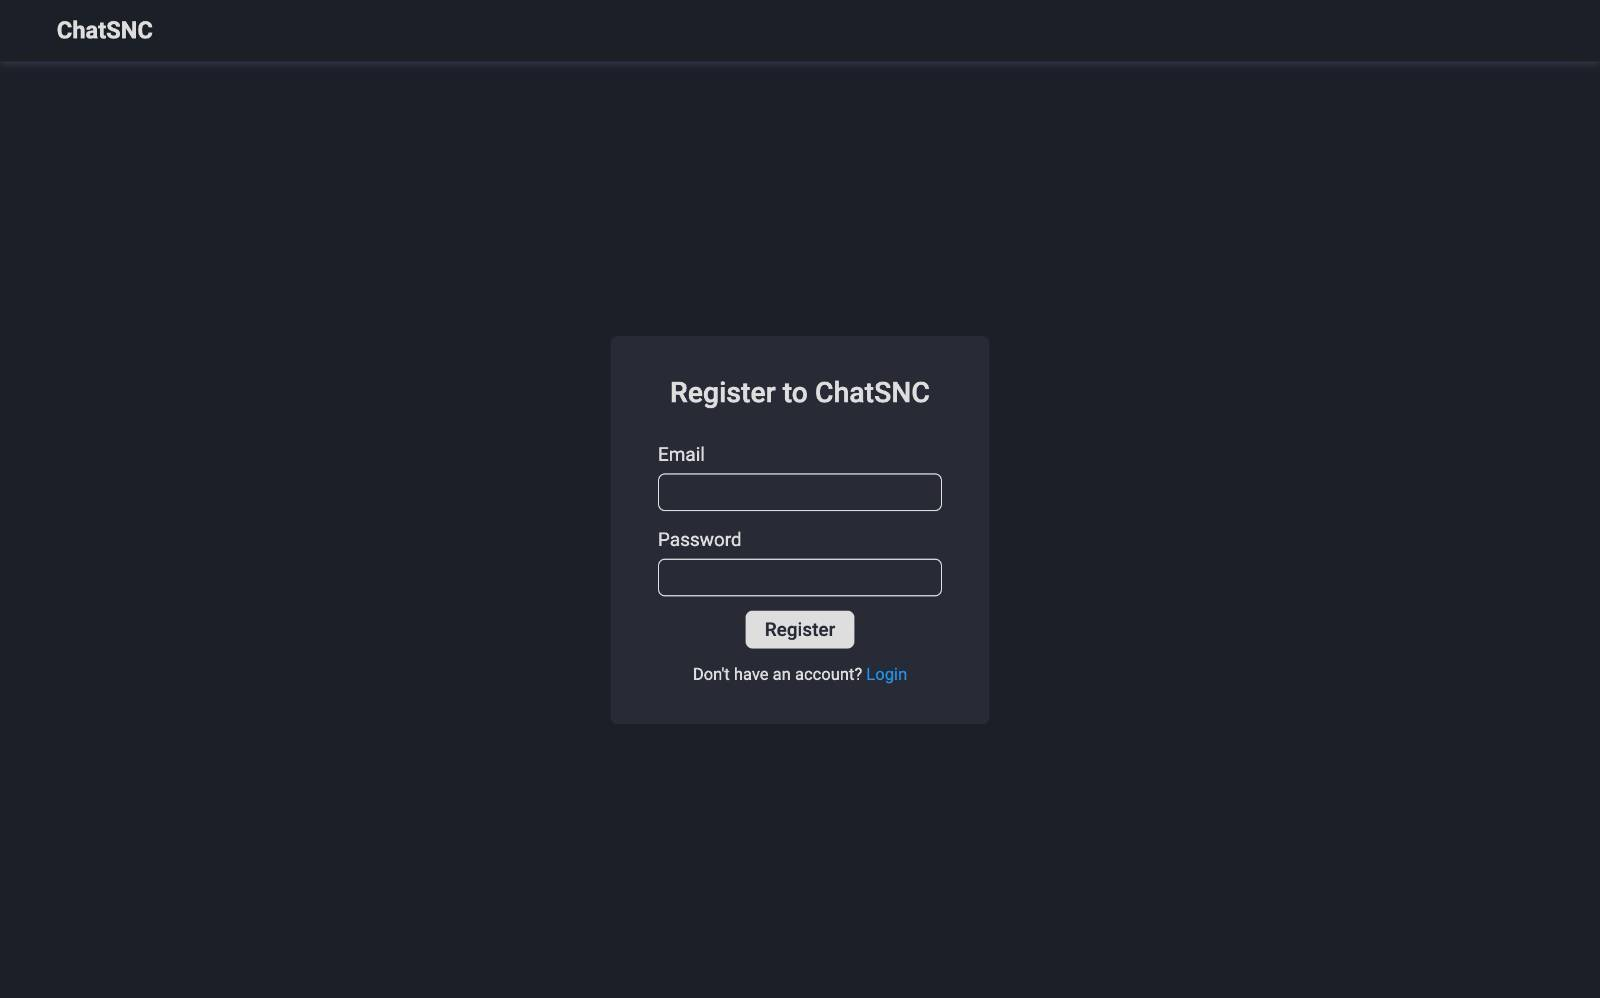
\includegraphics[width=\textwidth]{Register.png}
  \caption{Registration Screen}\label{fig:register}
\end{figure}

\begin{figure}[ht]
  \centering
  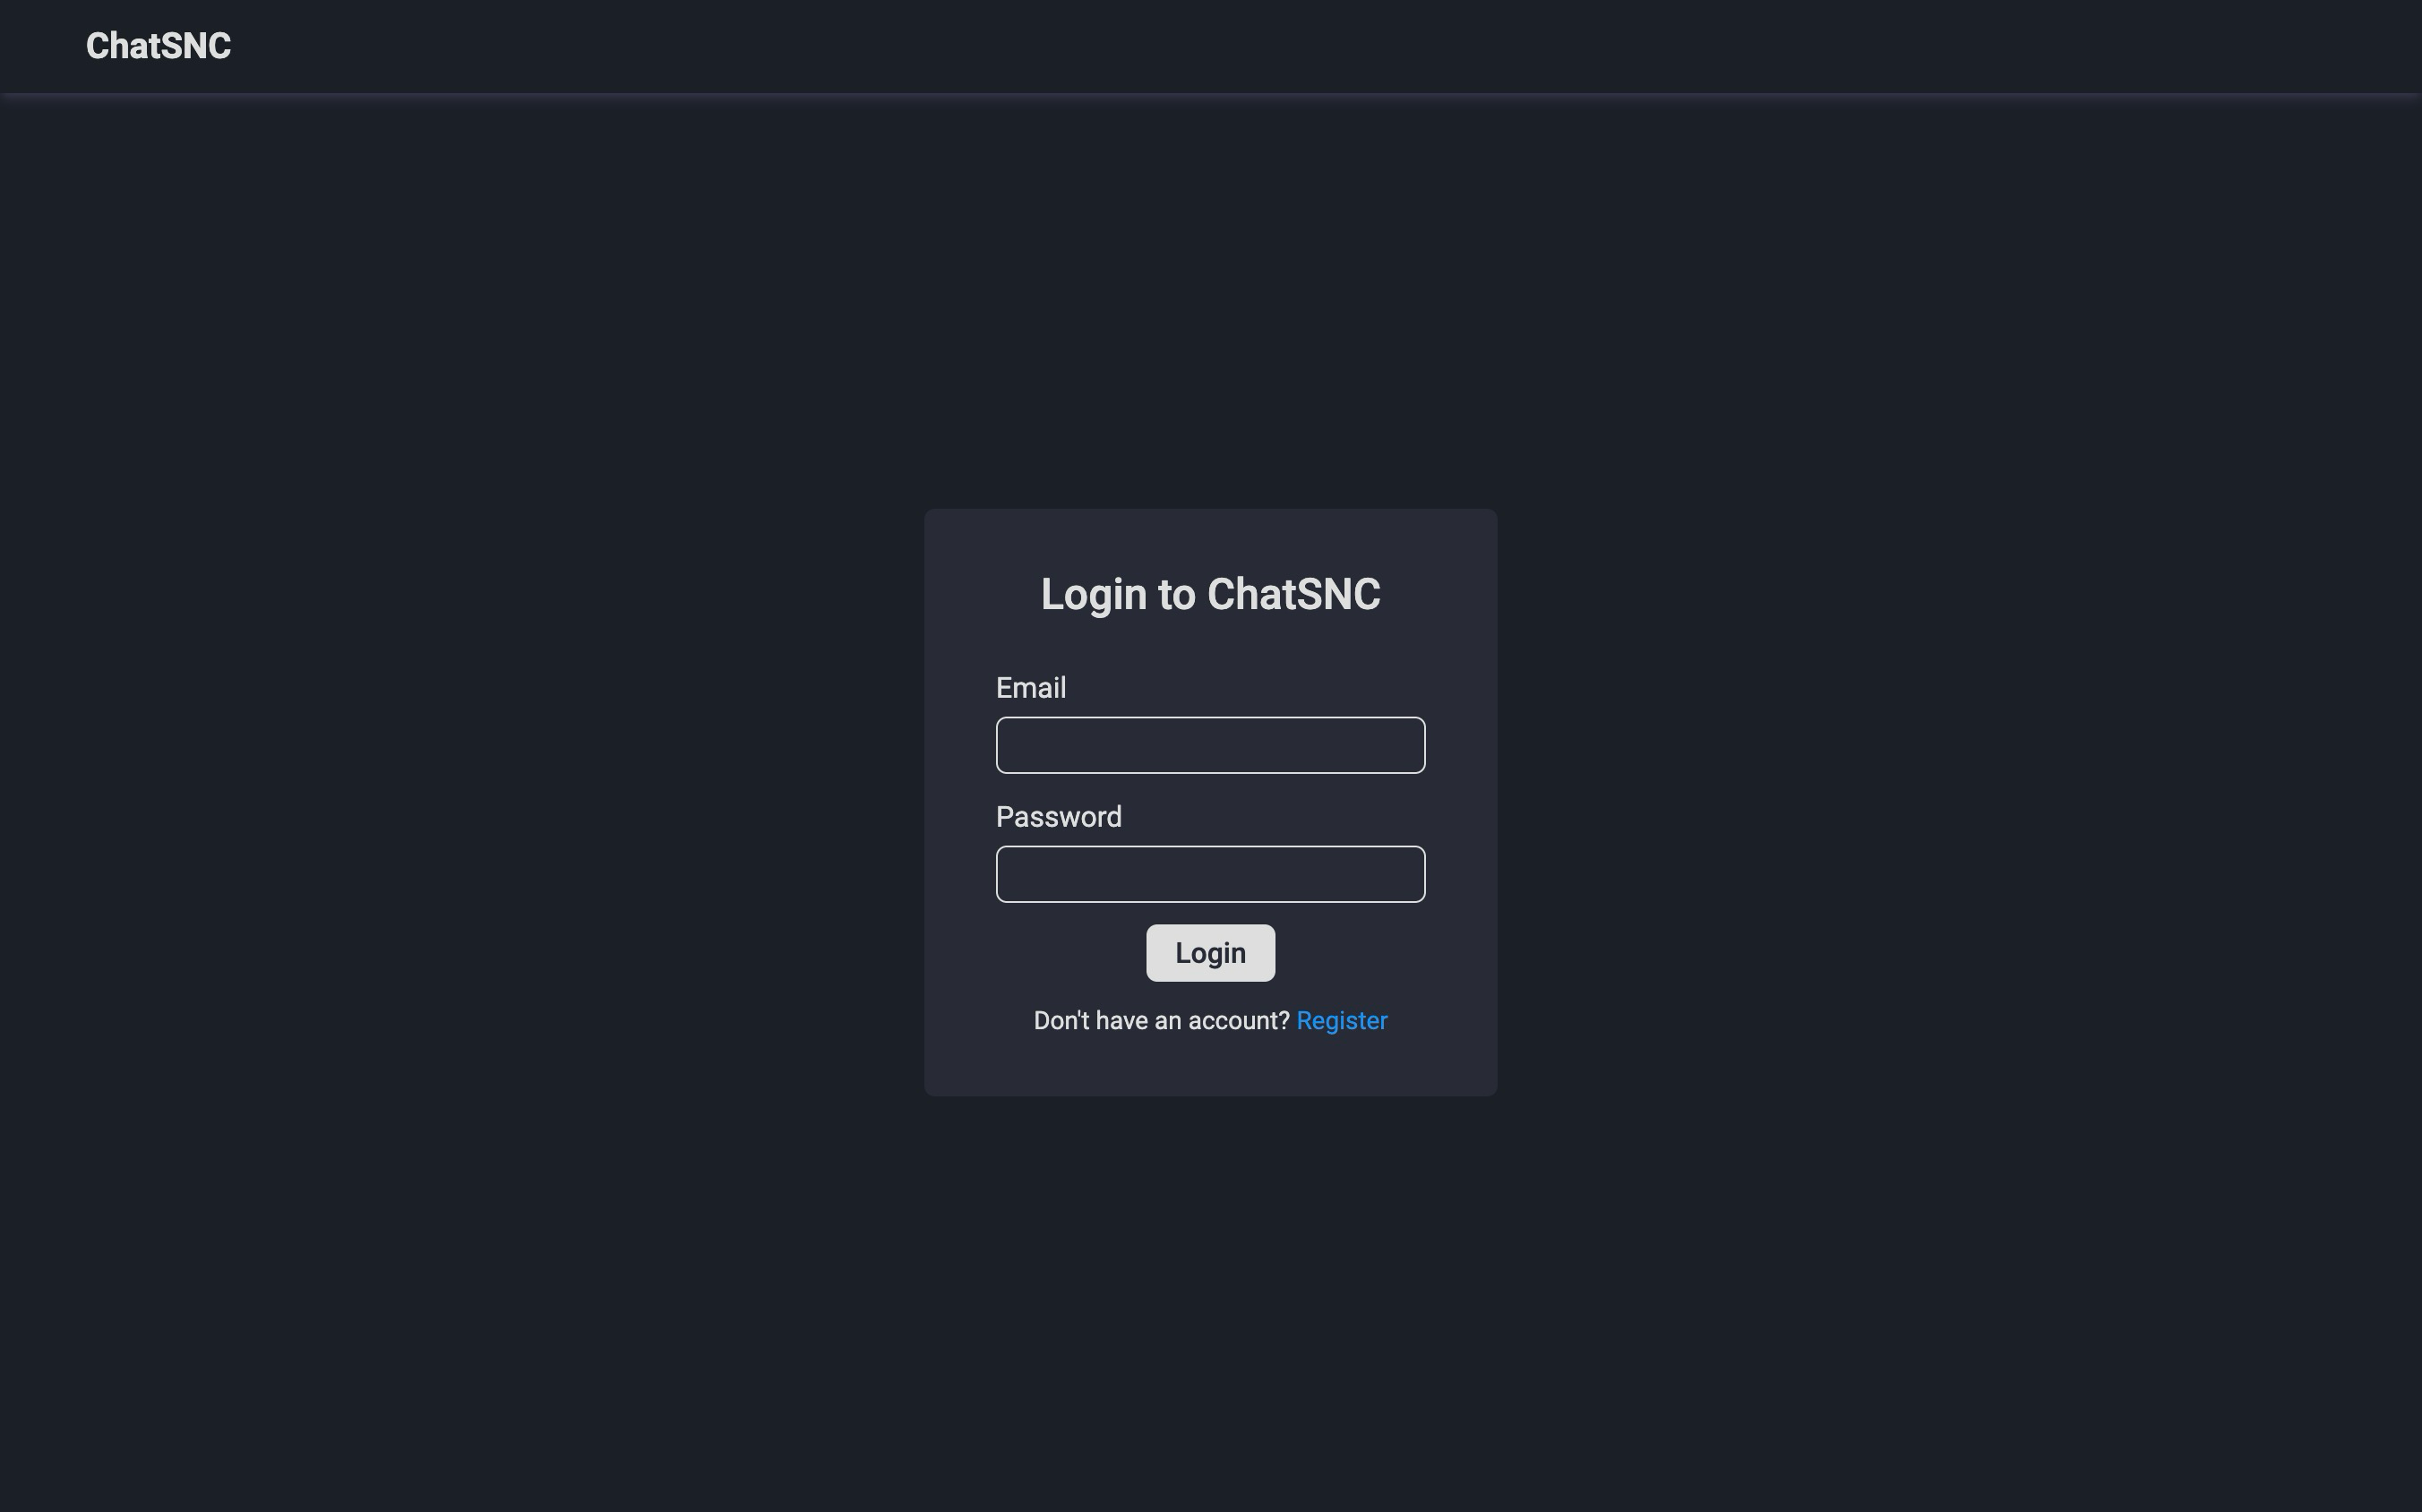
\includegraphics[width=\textwidth]{Login.png}
  \caption{Login Screen}\label{fig:login}
\end{figure}


\begin{figure}[ht]
  \centering
  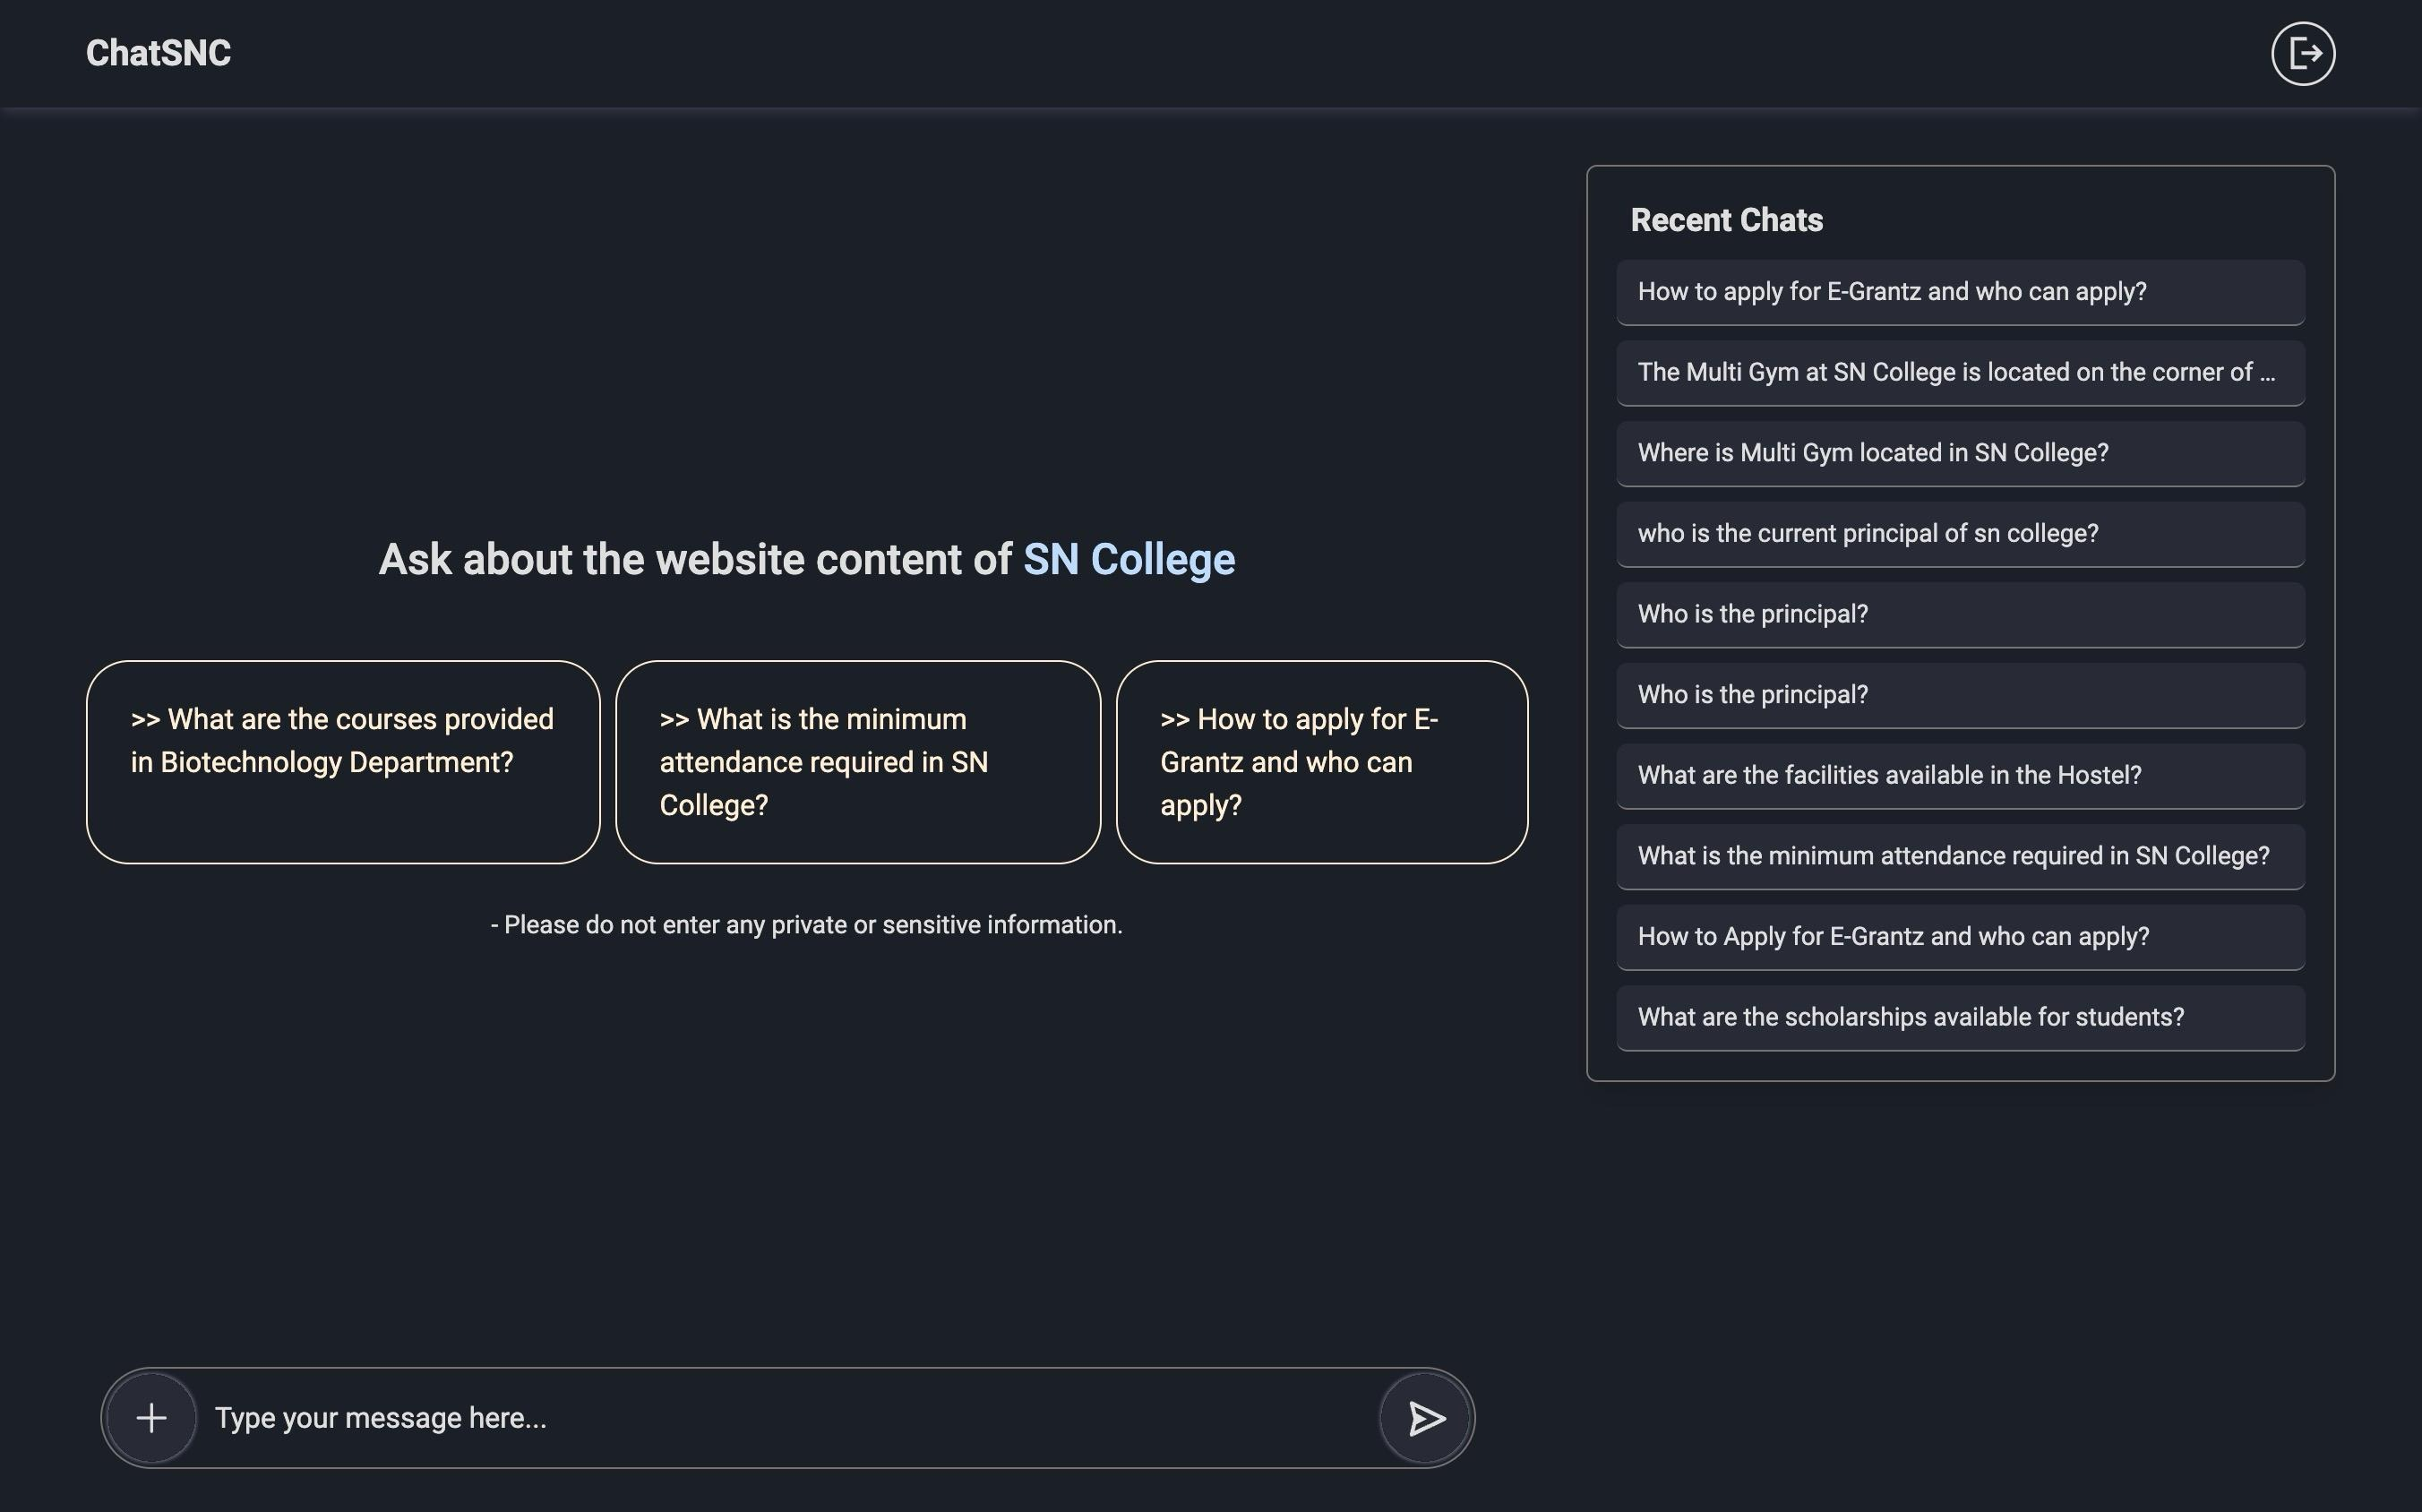
\includegraphics[width=\textwidth]{Opening_Screen.jpeg}
  \caption{Opening Screen}\label{fig:opening_screen}
\end{figure}

\begin{figure}[ht]
  \centering
  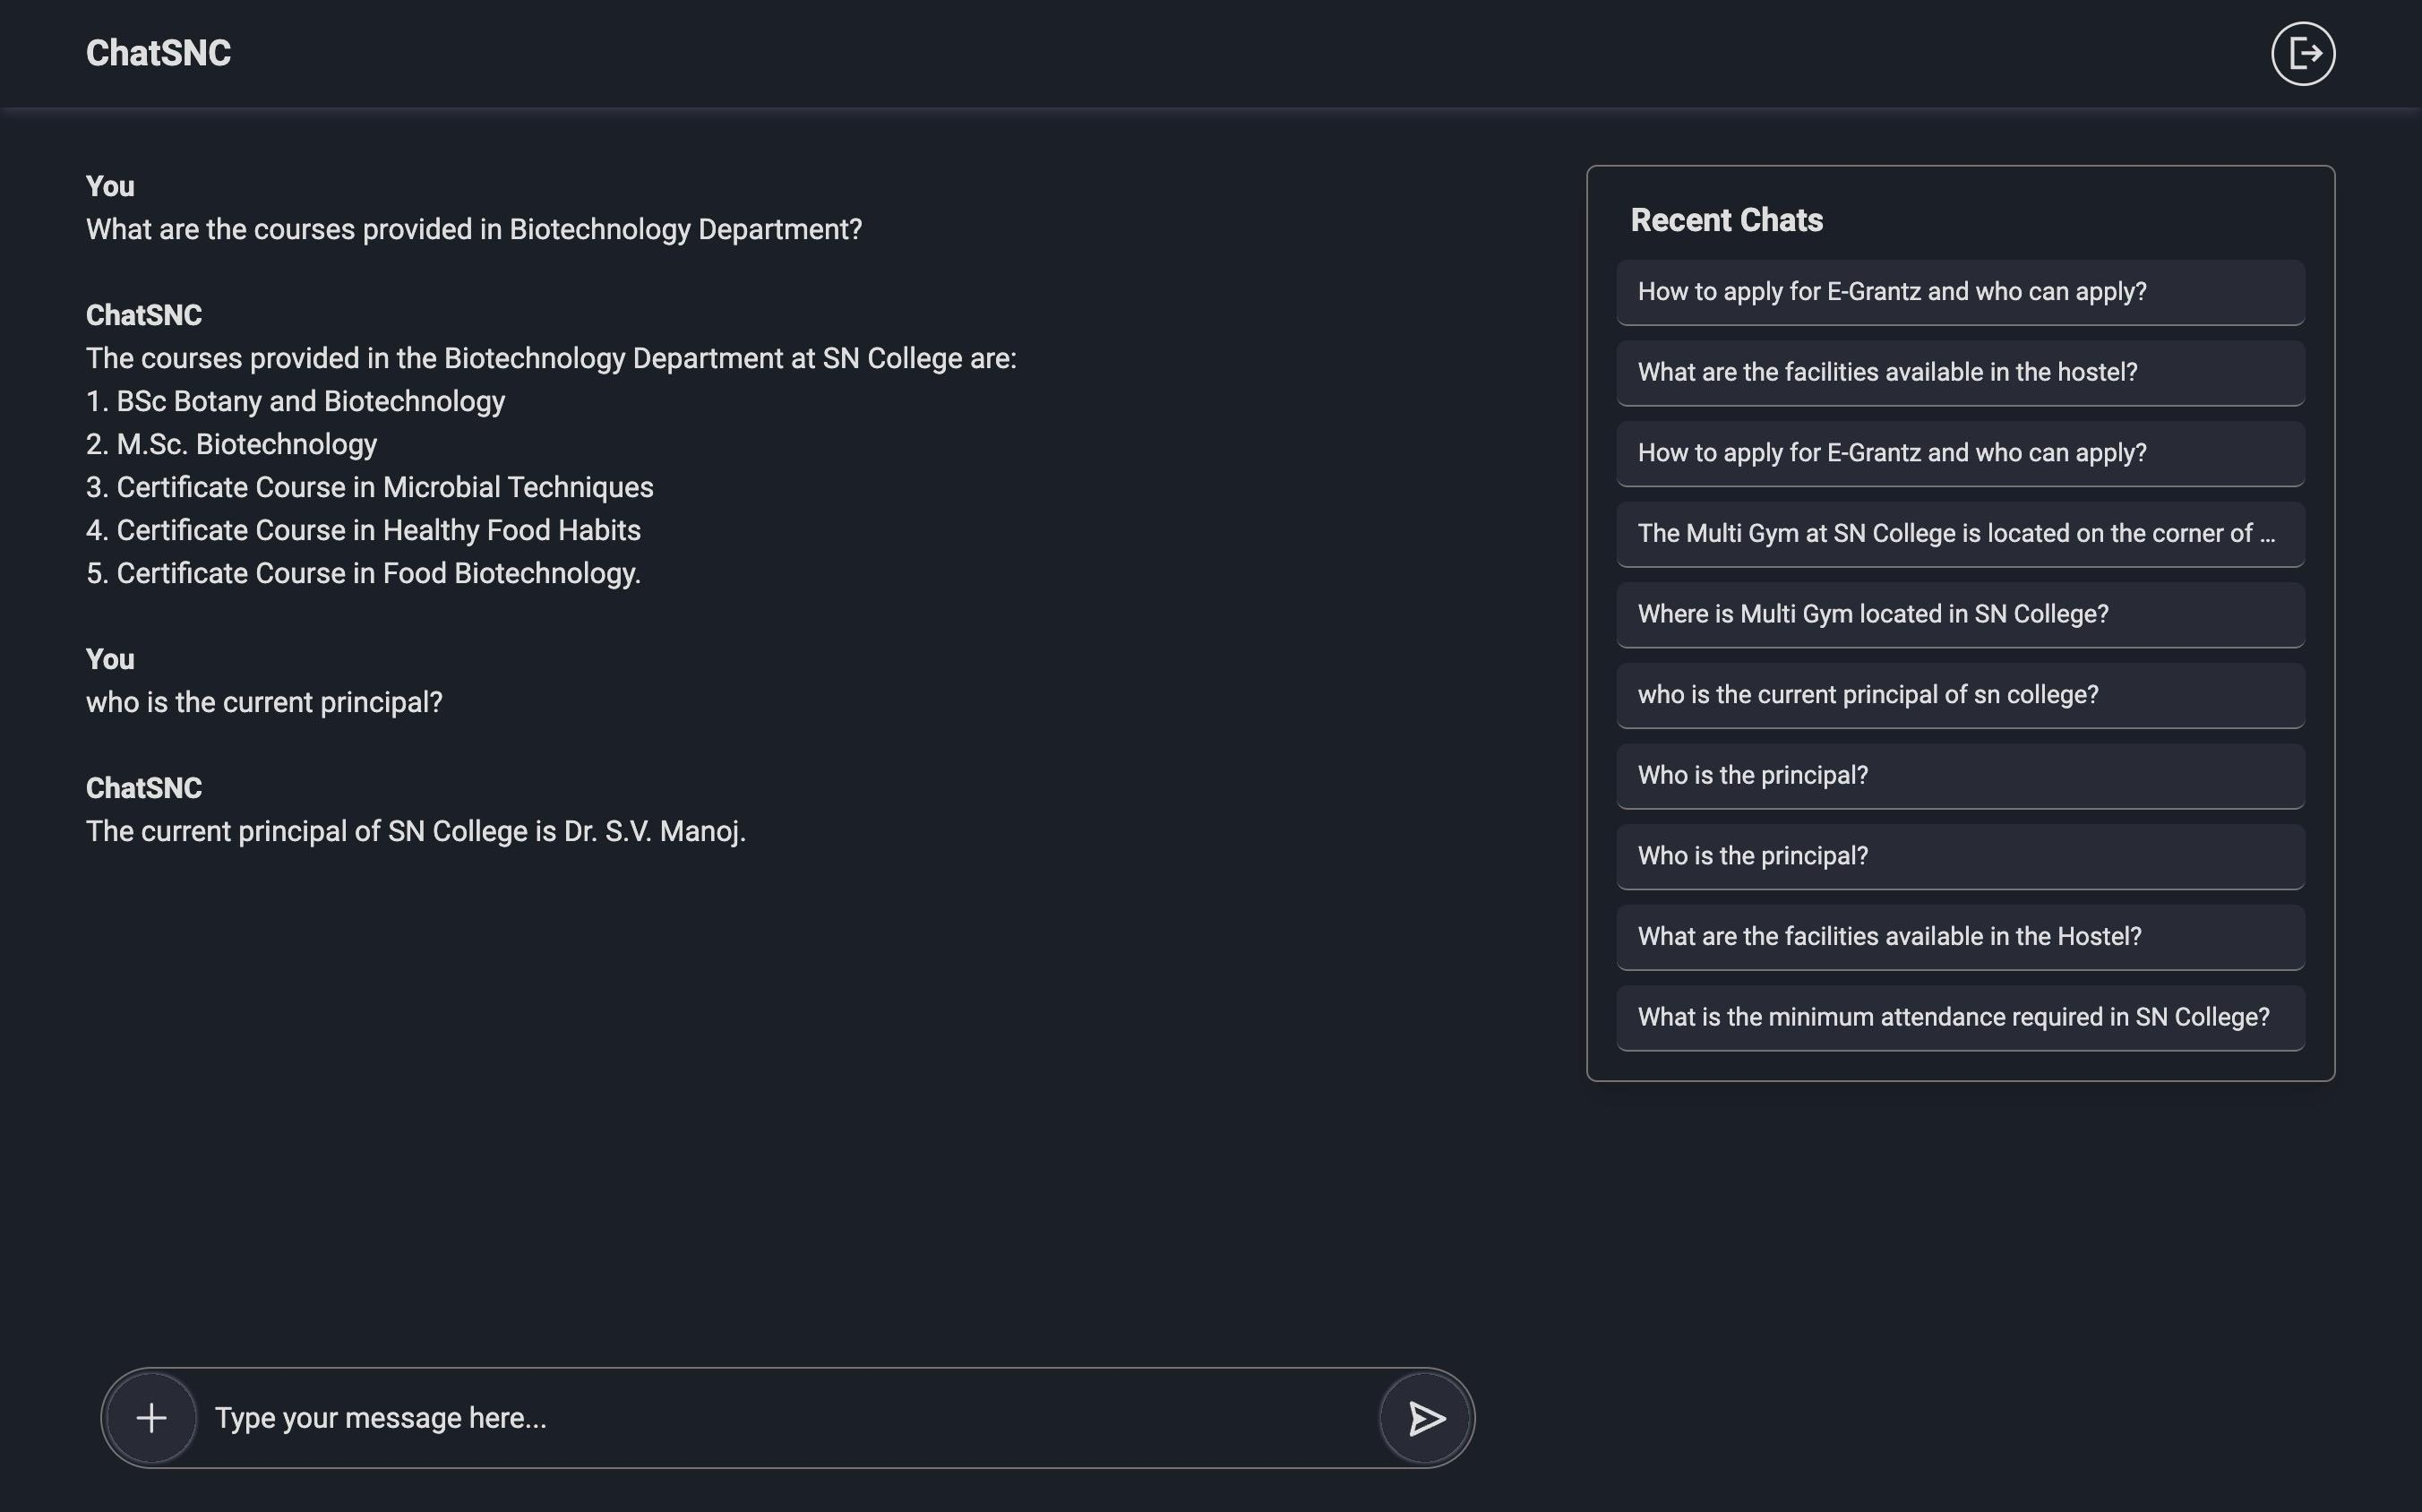
\includegraphics[width=\textwidth]{Chat_Screen.jpeg}
  \caption{Chat Screen}\label{fig:chat_screen}
\end{figure}



\bibliography{mybib}

\end{document}


